\section{Istruzioni per l'uso}
L'applicazione è composta da un'unica pagina web che prevede l'esecuzione di una serie operazioni ordinate da parte dell'utente:
\begin{itemize}
	\item Inserimento delle credenziali e generazione del captcha\textsubscript{G};
	\item Superamento del test captcha\textsubscript{G};
    \item Verifica delle credenziali e del superamento del test.
\end{itemize}    

\subsection{Inserimento delle credenziali e generazione del captcha\textsubscript{G}}
Una volta aperta la pagina web dell'applicazione viene visualizzata la pagina di login, dove l'utente deve:
\begin{itemize}
	\item Inserire l'username nell'apposito campo: \textbf{CatchEmAll};
	\item Inserire la password nell'apposito campo: \textbf{captcha};
    \item Premere il tasto \textbf{Genera captcha}.
\end{itemize}    
Per evitare un afflusso di richieste, prima di generare il captcha vengono verificate le credenziali. La richiesta verrà accettata solo nel caso queste ultime siano corrette.

\begin{figure}[H]
    \centering
    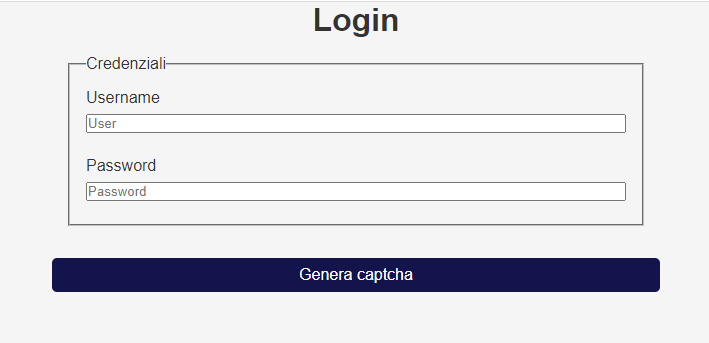
\includegraphics[scale=0.8]{img/login.png}
    \caption{Form di inserimento credenziali}
\end{figure}

\subsection{Superamento del test captcha\textsubscript{G}}
Il test captcha\textsubscript{G} è composto da due parti visibili all'utente:
\begin{itemize}
	\item Test immagini;
	\item Attesa operazioni in background\textsubscript{G}.
\end{itemize} 

\subsubsection{Test immagini}
Per poter essere riconosciuto come utente umano e non come un bot\textsubscript{G}, l'utente deve superare il test immagini. Questo test è composto da:
\begin{itemize}
    \item Una tipologia di immagini da selezionare;
	\item Una griglia 3x3 su cui sono disposte 9 immagini cliccabili, di cui solo alcune appartengono alla tipologia di immagine da selezionare.
\end{itemize} 

\begin{figure}[H]
    \centering
    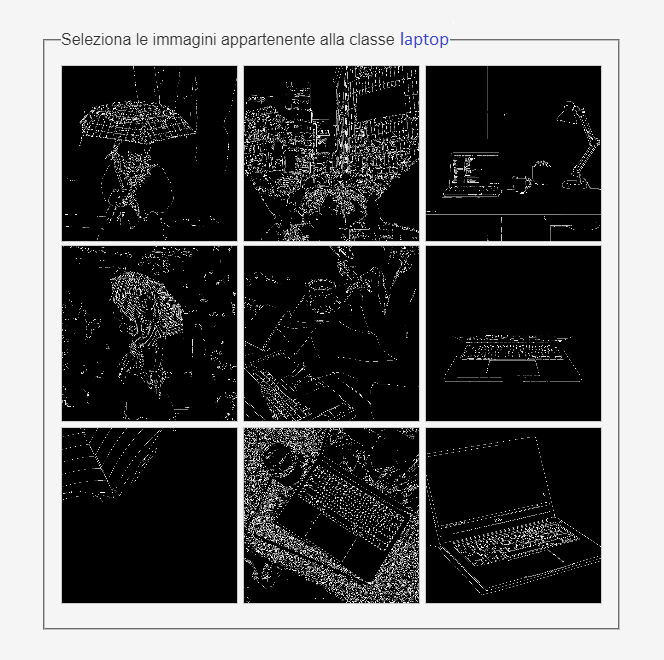
\includegraphics[scale=0.6]{img/captchaimg.png}
    \caption{Test immagini}
\end{figure}

\newpage
 
L'utente dovrà selezionare solo le immagini che ritiene facciano parte della tipologia richiesta - per esempio, nell'immagine sottostante è richiesto di selezionare le immagini appartenenti alla classe \textbf{laptop}, e le immagini corrette da selezionare vengono evidenziate in rosso:

\begin{figure}[H]
    \centering
    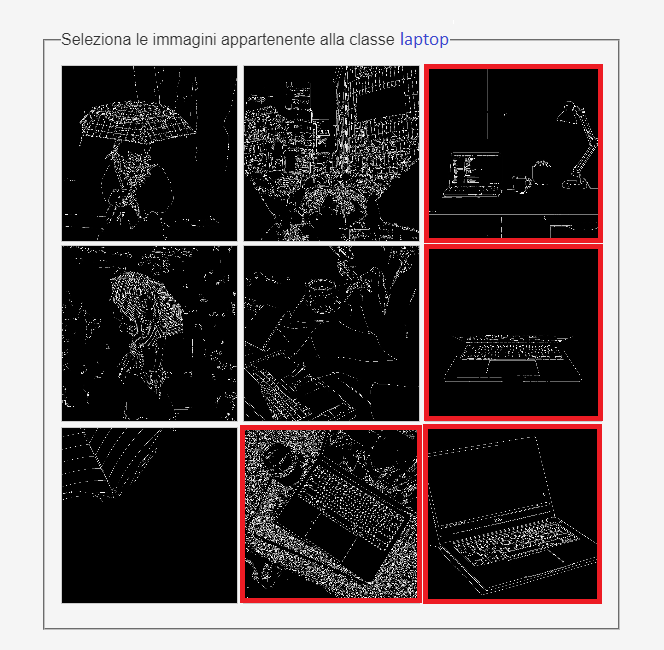
\includegraphics[scale=0.6]{img/captchaimgselezionato.png}
    \caption{Test immagini con soluzione evidenziata}
\end{figure}

\subsubsection{Attesa operazioni in background\textsubscript{G}}
L'utente per poter completare il captcha dovrà svolgere un proof of work, permettendoci di avere uno strato di sicurezza in più contro degli attacchi burst. Infatti si potrà procedere all'operazione successiva solo dopo che l'indicatore di progresso ha raggiunto il 100\%, come indicato nella seguente immagine:
\begin{figure}[H]
    \centering
    
\includegraphics[scale=0.8]{img/barra.png}
    \caption{Indicatore di progresso}
\end{figure} 

Osservazione:
\begin{itemize}
	\item Questa è un'operazione che richiede pochi secondi, e normalmente quando l'utente ha terminato la compilazione del test immagini l'avanzamento ha già raggiunto il 100\%.
\end{itemize}

\subsection{Verifica del test captcha}
Una volta effettuati i passaggi illustrati nei paragrafi precedenti, l'utente potrà procedere con l'autenticazione cliccando sul tasto \textbf{Login}. Se questa è andata a buon fine, l'utente verrà reindirizzato ad una pagina con un messaggio che indica la riuscita dell'operazione; altrimenti visualizzerà un messaggio di errore e potrà ritentare il login ripetendo i passaggi.

\begin{figure}[H]
    \centering
    
\includegraphics[scale=0.8]{img/tastologin.png}
    \caption{Pulsante di login}
\end{figure}

\begin{figure}[H]
	\centering
	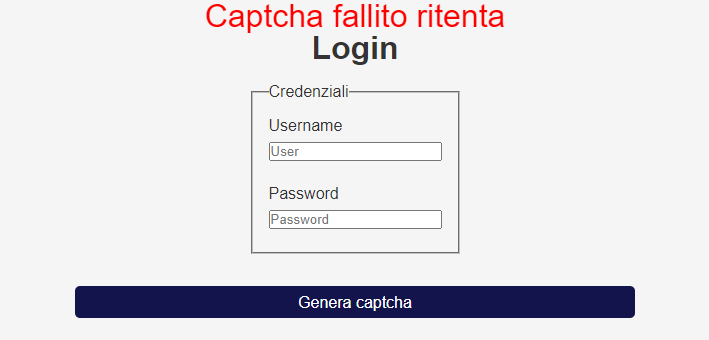
\includegraphics[scale=0.8]{img/message.png}
	\caption{Messaggio di errore}
\end{figure}   

\subsection{Problemi comuni}
Di seguito vengono elencati alcuni suggerimenti in merito alle operazioni alle quali prestare particolare attenzione nel caso in cui l'utente non riesca ad autenticarsi sul sistema:
\begin{itemize}
	\item L'utente non ha inserito correttamente le credenziali indicate al paragrafo \textbf{4.1};
    \item L'utente ha compilato erroneamente il test captcha\textsubscript{G} illustrato al paragrafo \textbf{4.2.2};
    \item L'utente non ha aspettato il completamento delle attività in background\textsubscript{G} come indicato al paragrafo \textbf{4.2.2}.
\end{itemize} 
